\documentclass[journal,12pt,twocolumn]{IEEEtran}

\usepackage{setspace}
\usepackage{textcomp,gensymb}
\singlespacing
\usepackage[cmex10]{amsmath}
\usepackage{enumerate}
\usepackage{amsmath}

\usepackage{amsthm}

\usepackage{mathrsfs}
\usepackage{txfonts}
\usepackage{stfloats}
\usepackage{bm}
\usepackage{cite}
\usepackage{cases}
\usepackage[caption=false]{subfig}

\usepackage{longtable}
\usepackage{multirow}



\usepackage{mathtools}
\usepackage{steinmetz}
\usepackage{tikz}


\usepackage{verbatim}
\usepackage{tfrupee}
\usepackage[breaklinks=true]{hyperref}
\usepackage{graphicx}
\usepackage{tkz-euclide}
\usepackage[rightcaption]{sidecap}


 
\graphicspath{ {images/} }


\usetikzlibrary{calc,math}
\usepackage{listings}
    \usepackage{color}                                            %%
    \usepackage{array}                                            %%
    \usepackage{longtable}                                        %%
    \usepackage{calc}                                             %%
    \usepackage{multirow}                                         %%
    \usepackage{hhline}                                           %%
    \usepackage{ifthen}                                           %%
    \usepackage{lscape}     


\DeclareMathOperator*{\Res}{Res}

\renewcommand\thesection{\arabic{section}}
\renewcommand\thesubsection{\thesection.\arabic{subsection}}
\renewcommand\thesubsubsection{\thesubsection.\arabic{sub-subsection}}

\renewcommand\thesectiondis{\arabic{section}}
\renewcommand\thesubsectiondis{\thesectiondis.\arabic{subsection}}
\renewcommand\thesubsubsectiondis{\thesubsectiondis.\arabic{sub-subsection}}


\hyphenation{op-ti-cal net-works semi-conduc-tor}
\def\inputGnumericTable{}                                 %%

\lstset{
%language=C,
frame=single, 
breaklines=true,
columns=fullflexible
}

\begin{document}


\newtheorem{theorem}{Theorem}[section]
\newtheorem{problem}{Problem}
\newtheorem{proposition}{Proposition}[section]
\newtheorem{lemma}{Lemma}[section]
\newtheorem{corollary}[theorem]{Corollary}
\newtheorem{example}{Example}[section]
\newtheorem{definition}[problem]{Definition}

\newcommand{\BEQA}{\begin{eqnarray}}
\newcommand{\EEQA}{\end{eqnarray}}
\newcommand{\define}{\stackrel{\triangle}{=}}
\bibliographystyle{IEEEtran}
\raggedbottom
\setlength{\parindent}{0pt}
\providecommand{\mbf}{\mathbf}
\providecommand{\pr}[1]{\ensuremath{\Pr\left(#1\right)}}
\providecommand{\qfunc}[1]{\ensuremath{Q\left(#1\right)}}
\providecommand{\sbrak}[1]{\ensuremath{{}\left[#1\right]}}
\providecommand{\lsbrak}[1]{\ensuremath{{}\left[#1\right.}}
\providecommand{\rsbrak}[1]{\ensuremath{{}\left.#1\right]}}
\providecommand{\brak}[1]{\ensuremath{\left(#1\right)}}
\providecommand{\lbrak}[1]{\ensuremath{\left(#1\right.}}
\providecommand{\rbrak}[1]{\ensuremath{\left.#1\right)}}
\providecommand{\cbrak}[1]{\ensuremath{\left\{#1\right\}}}
\providecommand{\lcbrak}[1]{\ensuremath{\left\{#1\right.}}
\providecommand{\rcbrak}[1]{\ensuremath{\left.#1\right\}}}
\theoremstyle{remark}
\newtheorem{rem}{Remark}
\newcommand{\sgn}{\mathop{\mathrm{sgn}}}
\providecommand{\res}[1]{\Res\displaylimits_{#1}} 
%\providecommand{\norm}[1]{\lVert#1\rVert}
\providecommand{\mtx}[1]{\mathbf{#1}}
\providecommand{\fourier}{\overset{\mathcal{F}}{ \rightleftharpoons}}
\providecommand{\hilbert}{\overset{\mathcal{H}}{ \rightleftharpoons}}
\providecommand{\system}{\overset{\mathcal{H}}{ \longleftrightarrow}}
	\newcommand{\solution}[2]{\textbf{Solution:}{#1}}
%\newcommand{\cosec}{\,\text{cosec}\,}
\providecommand{\dec}[2]{\ensuremath{\overset{#1}{\underset{#2}{\gtrless}}}}
\newcommand{\myvec}[1]{\ensuremath{\begin{pmatrix}#1\end{pmatrix}}}
\newcommand{\mydet}[1]{\ensuremath{\begin{vmatrix}#1\end{vmatrix}}}
\numberwithin{equation}{subsection}
\makeatletter
\@addtoreset{figure}{problem}
\makeatother
\let\StandardTheFigure\thefigure
\let\vec\mathbf
\renewcommand{\thefigure}{\theproblem}
\def\putbox#1#2#3{\makebox[0in][l]{\makebox[#1][l]{}\raisebox{\baselineskip}[0in][0in]{\raisebox{#2}[0in][0in]{#3}}}}
     \def\rightbox#1{\makebox[0in][r]{#1}}
     \def\centbox#1{\makebox[0in]{#1}}
     \def\topbox#1{\raisebox{-\baselineskip}[0in][0in]{#1}}
     \def\midbox#1{\raisebox{-0.5\baselineskip}[0in][0in]{#1}}
\vspace{3cm}
\title{Assignment 1}
\author{Prabhath Chellingi - CS20BTECH11038}
\maketitle
\newpage
\bigskip
\renewcommand{\thefigure}{\theenumi}
\renewcommand{\thetable}{\theenumi}

Download all python codes from 
\begin{lstlisting}
https://github.com/PRABHATH-cs20-11038/Assignment_1/tree/main/Assignment_1/Codes
\end{lstlisting}

and latex-tikz codes from
\begin{lstlisting}
https://github.com/PRABHATH-cs20-11038/Assignment_1/blob/main/Assignment_1/Assignment_1.tex
\end{lstlisting}

\section{Problem}
(Prob 3.6) Find the probability distribution of

(i) number of heads in two tosses of a coin.

(ii) number of tails in the simultaneous tosses of three coins.

(iii) number of heads in four tosses of a coin.
\section{Solution}

Let $X_i \in \{0, 1\}$ represent the $i^{Th}$ coin where 1 denotes the coin giving outcome as head. Then, $X_i$ has a Bernoulli distribution with parameter
\begin{align}
p = \frac{1}{2}
\end{align}

Let 
\begin{align}
X = \sum\limits_{i=1}^{n}X_i
\end{align}

where n is the total number of coins tossed. Then $X$ has a Binomial Distribution. Then for 
\begin{align}
    \pr{X_i=n} {\stackrel{Z}{\rightleftharpoons}} \pr{X_i=z}
\end{align}

yielding
\begin{align}
    \pr{X_i=z} = 1-p+p z^{-1}
\end{align}

with using the fact that $X_i$ are i.i.d.,
\begin{align}
\begin{split}
    \pr{X=z} &= (1-p+p z^{-1})^n\\
    &=\sum\limits_{k=0}^n{^n C_k}p^k(1-p)^{n-k}z^{-k}
\end{split}
\end{align}

\begin{align}\label{eq1}
   \pr{X=k} =
  \begin{cases*}
    {^n C_k}p^{k}(1-p)^{n-k} & $0 \leq k \leq n$\\
      0 & otherwise
  \end{cases*}
\end{align}

\begin{table}[h!]
\centering
\caption{Table of Probability distribution of different cases}
\resizebox{.5\textwidth}{!}{
  \begin{tabular}{|c|m{1cm}|m{2cm}|c|c|c|c|c|}
  \hline
    Case &  n (no. of coins) & k (no. of required outcomes) & 0 & 1 & 2 & 3 & 4\\
    \hline
    $(i)$ & 2 & $\pr{X=k}={^2 C_k}\brak{\frac{1}{2}}^{2}$ & $1/2$& $1/4$ & $1/2$ & $0$ & $0$\\
    \hline
    $(ii)$ & 3 & $\pr{X=k}={^3 C_k}\brak{\frac{1}{2}}^{3}$ & $1/8$ & $3/8$ & $3/8$ & $1/8$ & $0$\\
    \hline
    $(iii)$ & 4 & $\pr{X=k}={^4 C_k}\brak{\frac{1}{2}}^{4}$ & $1/16$& $1/4$ & $3/8$ & $1/4$ & $1/16$\\
    \hline
  \end{tabular}
  \label{Table1}
}
\end{table}

The above table represents the probability distribution of following cases at different $k$ values.

\begin{enumerate}[(i)]
    \item from \eqref{eq1}
\begin{align}
   \pr{X=k} =
  \begin{cases*}
    {^2 C_k}\brak{\frac{1}{2}}^{2} \quad& if $0 \leq k \leq 2$ \\
    0 \quad& otherwise
  \end{cases*}
\end{align}

\begin{figure}[h!]
    \centering
    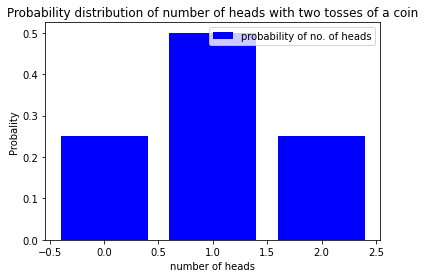
\includegraphics[width=\linewidth]{Figure_1.png}
    \caption{Plot of probability distribution of two tossed coins}
    \label{fig:Two coins}
\end{figure}

\vspace{0.2in}

\item probability of tails,

from \eqref{eq1}
\begin{align}\label{eq2}
   \pr{X=k} =
  \begin{cases*}
    {^n C_k}(p)^{n-k}(1-p)^{k} & $0 \leq k \leq n$\\
      0 & otherwise
  \end{cases*}
\end{align}

 from \eqref{eq2},

\begin{align}
   \pr{X=k} =
  \begin{cases*}
    {^3 C_k}\brak{\frac{1}{2}}^{3} \quad& if $0 \leq k \leq 3$ \\
    0 \quad& otherwise
  \end{cases*}
\end{align}

\begin{figure}[h!]
    \centering
    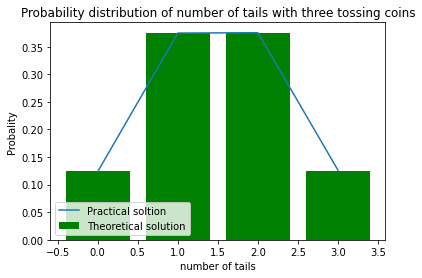
\includegraphics[width=\linewidth]{Figure_2.png}
    \caption{Plot of probability distribution of no of tails with three tossed coins}
    \label{fig:Three coins}
\end{figure}

\item 
from \eqref{eq1},
\begin{align}
   \pr{X=k} =
  \begin{cases*}
    {^4 C_k}\brak{\frac{1}{2}}^{4} \quad& if $0 \leq k \leq 4$ \\
    0 \quad& otherwise
  \end{cases*}
\end{align}

\begin{figure}[h!]
    \centering
    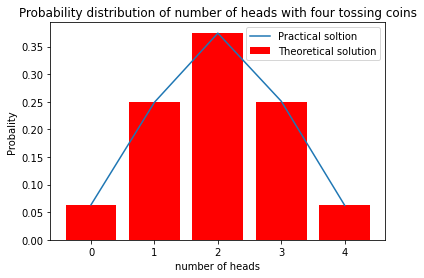
\includegraphics[width=\linewidth]{Figure_3.png}
    \caption{Plot of probability distribution of four tossed coins}
    \label{fig:Four coins}
\end{figure}

\end{enumerate}

\end{document}
